\documentclass[a4paper,12pt]{article}
\usepackage{amsmath}
\usepackage{graphicx}
\graphicspath{ {images/} }
\usepackage{float}
\usepackage[utf8]{inputenc}
\usepackage[english]{babel}
\usepackage[document]{ragged2e}
\usepackage{mathpazo}
\usepackage{rotating}
 
\begin{document}\begin{flushleft}\newline \textbf{6.819 PSET 8}
\newline \textbf{11/17/2017}
\end{flushleft}
\newline \begin{center}\textbf{ISAAC KONTOMAH}
\end{center}
\begin{flushleft}
\newline \emph{Collaborators: Kamoya Ikhofua,Benjamin Waar,Afika Nyati ,Andrew Zhang, Abishkar Chhetri,Suman Nepal}
\end{flushleft}

\section{\emph{\textbf{ Markov Network}}}
\newline $a.$
\[
   \phi(a,d)=\phi(c,e)=
  \left[ {\begin{array}{cc}
   0.9 & 0.1 \\
   0.9 & 0.9 \\
  \end{array} } \right]
\]
\[
   \psi(a,b)=\psi(b,c)=
  \left[ {\begin{array}{cc}
   \alpha & 1-\alpha \\
   1-\alpha & \alpha \\
  \end{array} } \right]
\]
\newline $n_{p}$ denote node potential
\newline $n_{p}(d)=\[
  \left[ {\begin{array}{c}
   0\\
   1\\
  \end{array} } \right]
\]
\newline $n_{p}(a)=\[
  \left[ {\begin{array}{c}
   1\\
   0\\
  \end{array} } \right]
\]
\newline $P(a)=M_{d \rightarrow a}M_{b \rightarrow a}$
\newline $M_{d \rightarrow a}=\phi(d,a)n_{p}(d)=\left[ {\begin{array}{cc}
   0.9 & 0.1 \\
   0.9 & 0.9 \\
  \end{array} } \right] \left[ {\begin{array}{c}
   0\\
   1\\
  \end{array} } \right]= \left[ {\begin{array}{c}
   0.1\\
   0.9\\
  \end{array} } \right]$,
  \newline hence ,$M_{d \rightarrow a}=   \end{array} } \right]= \left[ {\begin{array}{c}
   0.1\\
   0.9\\
  \end{array} } \right]$
\newline $M_{e \rightarrow c}=\phi(e,c)=\phi(c,e)n_{p}(e)=
  \left[ {\begin{array}{cc}
   0.9 & 0.1 \\
   0.9 & 0.9 \\
  \end{array} } \right] \left[ {\begin{array}{c}
   1\\
   0\\
  \end{array} } \right]= \left[ {\begin{array}{c}
   0.9\\
   0.1\\
  \end{array} } \right]
  $
  \newline $M_{c \rightarrow b}=\psi(c,b)n_{p}(c) , $
  \newline$n_{p}(c)=M_{e \rightarrow c} \times   \left[ {\begin{array}{c}
   1\\
   1\\
  \end{array} } \right]=\left[ {\begin{array}{c}
   0.9\\
   0.1\\
  \end{array} } \right]$
 \newline  $M_{c \rightarrow b}=\left[ {\begin{array}{cc}
   0.99 & 0.01 \\
   0.01 & 0.99 \\
  \end{array} } \right] \left[ {\begin{array}{c}
   0.9\\
   0.1\\
  \end{array} } \right]= \left[ {\begin{array}{c}
   0.892\\
   0.108\\
  \end{array} } \right]$
  \newline $M_{b \rightarrow a}=\psi(b,a)n_{p}(b) , $
  \newline$n_{p}(b)=M_{c \rightarrow b} \times   \left[ {\begin{array}{c}
   1\\
   1\\
  \end{array} } \right]=\left[ {\begin{array}{c}
   0.892\\
   0.108\\
  \end{array} } \right]$
 \newline  $M_{b \rightarrow a}=\left[ {\begin{array}{cc}
   0.99 & 0.01 \\
   0.01 & 0.99 \\
  \end{array} } \right] \left[ {\begin{array}{c}
   0.892\\
   0.108\\
  \end{array} } \right]= \left[ {\begin{array}{c}
   0.88416\\
   0.11584\\
  \end{array} } \right]$
  \newline $P(a)=M_{d \rightarrow a}M_{b \rightarrow a}=\left[ {\begin{array}{c}
   0.1\\
   0.9\\
  \end{array} } \right]\left[ {\begin{array}{c}
   0.88416\\
   0.11584\\
  \end{array} } \right]=\left[ {\begin{array}{c}
   0.088416\\
   0.104256\\
  \end{array} } \right]$
  \newline Normalizing the values , $P(a)=\left[ {\begin{array}{c}
   \frac{0.088416}{0.192672\\
  \frac{0.104256}{0.192672}\\
  \end{array} } \right]=\left[ {\begin{array}{c}
  0.459\\
  0.541\\
  \end{array} } \right]$
  
  
  \newline $b.$
  
  \[
   \phi(a,d)=\phi(c,e)=
  \left[ {\begin{array}{cc}
   0.9 & 0.1 \\
   0.9 & 0.9 \\
  \end{array} } \right]
\]
\[
   \psi(a,b)=\psi(b,c)=
  \left[ {\begin{array}{cc}
   \alpha & 1-\alpha \\
   1-\alpha & \alpha \\
  \end{array} } \right]
\]
\newline $n_{p}$ denote node potential
\newline $n_{p}(d)=\[
  \left[ {\begin{array}{c}
   0\\
   1\\
  \end{array} } \right]
\]
\newline $n_{p}(a)=\[
  \left[ {\begin{array}{c}
   1\\
   0\\
  \end{array} } \right]
\]
\newline $P(a)=M_{d \rightarrow a}M_{b \rightarrow a}$
\newline $M_{d \rightarrow a}=\phi(d,a)n_{p}(d)=\left[ {\begin{array}{cc}
   0.9 & 0.1 \\
   0.9 & 0.9 \\
  \end{array} } \right] \left[ {\begin{array}{c}
   0\\
   1\\
  \end{array} } \right]= \left[ {\begin{array}{c}
   0.1\\
   0.9\\
  \end{array} } \right]$,
  \newline hence ,$M_{d \rightarrow a}=   \end{array} } \right]= \left[ {\begin{array}{c}
   0.1\\
   0.9\\
  \end{array} } \right]$
\newline $M_{e \rightarrow c}=\phi(e,c)=\phi(c,e)n_{p}(e)=
  \left[ {\begin{array}{cc}
   0.9 & 0.1 \\
   0.9 & 0.9 \\
  \end{array} } \right] \left[ {\begin{array}{c}
   1\\
   0\\
  \end{array} } \right]= \left[ {\begin{array}{c}
   0.9\\
   0.1\\
  \end{array} } \right]
  $
  \newline $M_{c \rightarrow b}=\psi(c,b)n_{p}(c) , $
  \newline$n_{p}(c)=M_{e \rightarrow c} \times   \left[ {\begin{array}{c}
   1\\
   1\\
  \end{array} } \right]=\left[ {\begin{array}{c}
   0.9\\
   0.1\\
  \end{array} } \right]$
 \newline  $M_{c \rightarrow b}=\left[ {\begin{array}{cc}
   0.6 & 0.4 \\
   0.4 & 0.6 \\
  \end{array} } \right] \left[ {\begin{array}{c}
   0.9\\
   0.1\\
  \end{array} } \right]= \left[ {\begin{array}{c}
   0.58\\
   0.42\\
  \end{array} } \right]$
  \newline $M_{b \rightarrow a}=\psi(b,a)n_{p}(b) , $
  \newline$n_{p}(b)=M_{b \rightarrow a} \times   \left[ {\begin{array}{c}
   1\\
   1\\
  \end{array} } \right]=\left[ {\begin{array}{c}
   0.58\\
   0.42\\
  \end{array} } \right]$
 \newline  $M_{b \rightarrow a}=\left[ {\begin{array}{cc}
   0.6 & 0.4 \\
   0.4 & 0.6 \\
  \end{array} } \right] \left[ {\begin{array}{c}
   0.58\\
   0.42\\
  \end{array} } \right]= \left[ {\begin{array}{c}
   0.516\\
   0.484\\
  \end{array} } \right]$
  \newline $P(a)=M_{d \rightarrow a}M_{b \rightarrow a}=\left[ {\begin{array}{c}
   0.1\\
   0.9\\
  \end{array} } \right]\left[ {\begin{array}{c}
   0.516\\
   0.484\\
  \end{array} } \right]=\left[ {\begin{array}{c}
   0.0516\\
   0.4356\\
  \end{array} } \right]$
   \newline Normalizing the values , $P(a)=\left[ {\begin{array}{c}
   \frac{0.0516}{0.4872}\\
  \frac{0.484}{0.4872}\\
  \end{array} } \right]=\left[ {\begin{array}{c}
  0.1059\\
  0.8941\\
  \end{array} } \right]$
  \newline \emph{\textbf{Explanation of difference in results}}
  \newline The marginal probabilities of $P(a)$ being in its different states , state $0$ and $1$ are almost quite likely when $\alpha=0.99$ but very far apart when $\alpha=0.6$.This is because the transition matrix multiplies the node potential at each node to update the node potential before a message is then passed among the edge connecting the two nodes , hence a higher $\alpha$ value means there is higher compatibility between the states and the node will more on less prefer to be in any of the two , but a lesser value of $\alpha$ will mean it has lesser compatibility hence will prefer one state over the other.
\section{\emph{\textbf{ Belief Propagation}}}
\newline $a.$
\newline \begin{document}
\newline Flower Contours

 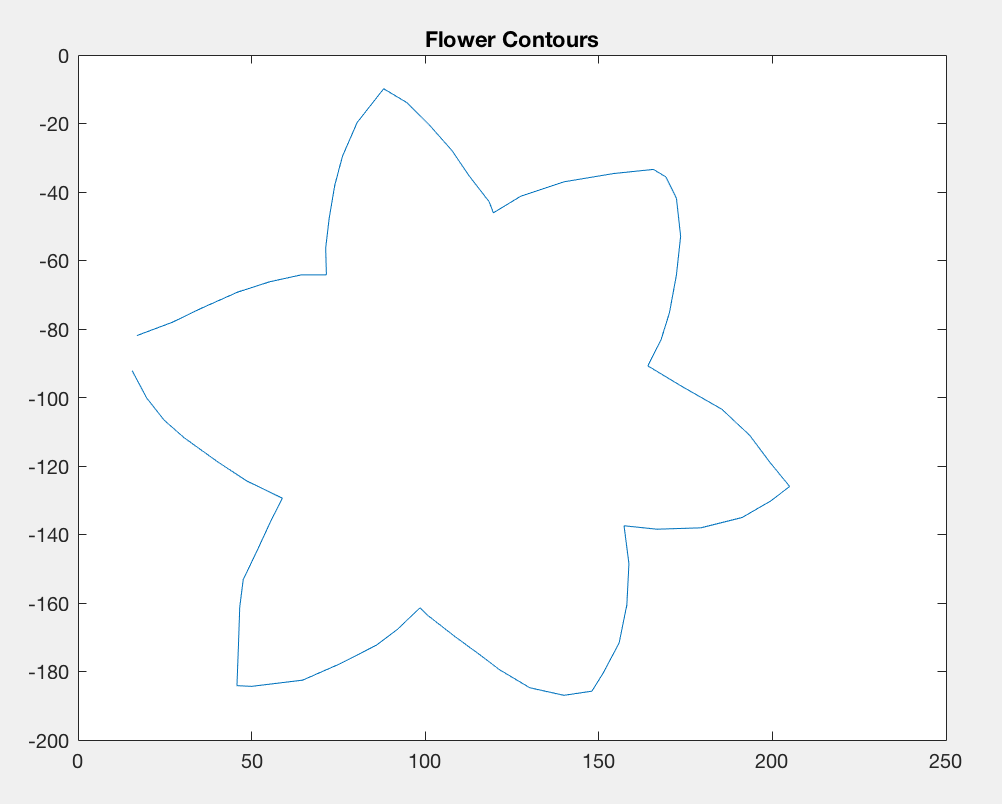
\includegraphics[height=5cm , width=8cm]{flower.jpg}

 \emph{Image showing contours of flower image}
 \newline \begin{document}
\newline Hand Contours

 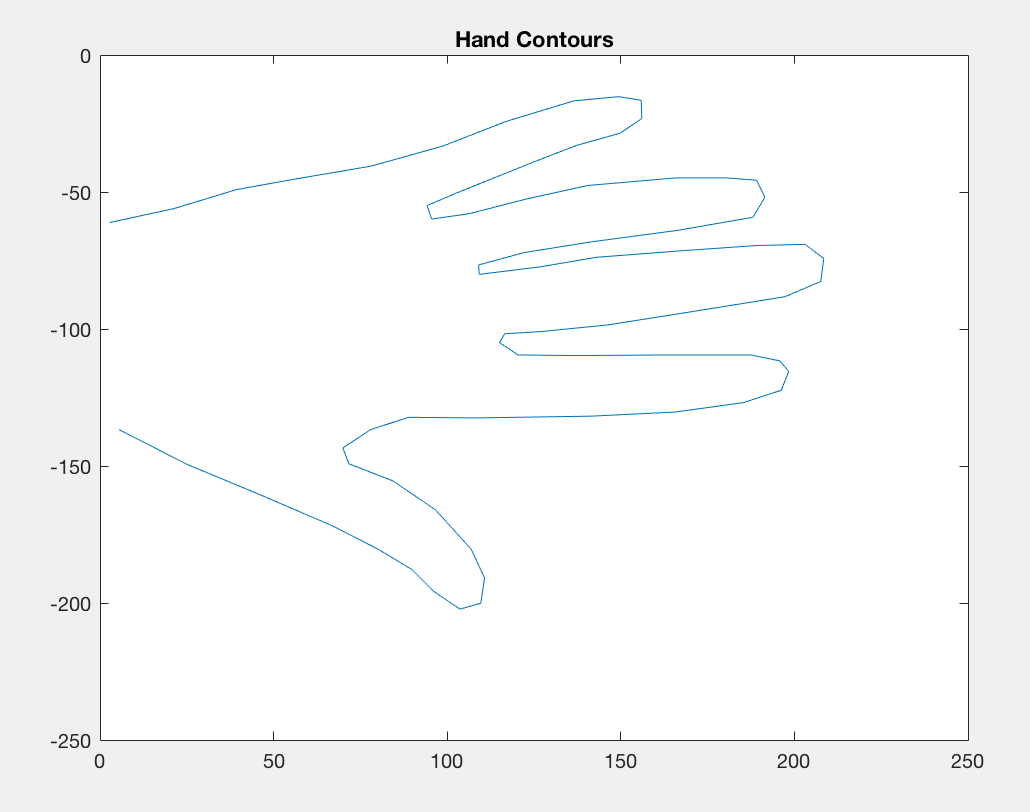
\includegraphics[height=5cm , width=8cm]{hand.jpg}

 \emph{Image showing contours of hand}
  \newline \begin{document}
\newline Pedestrian contours

 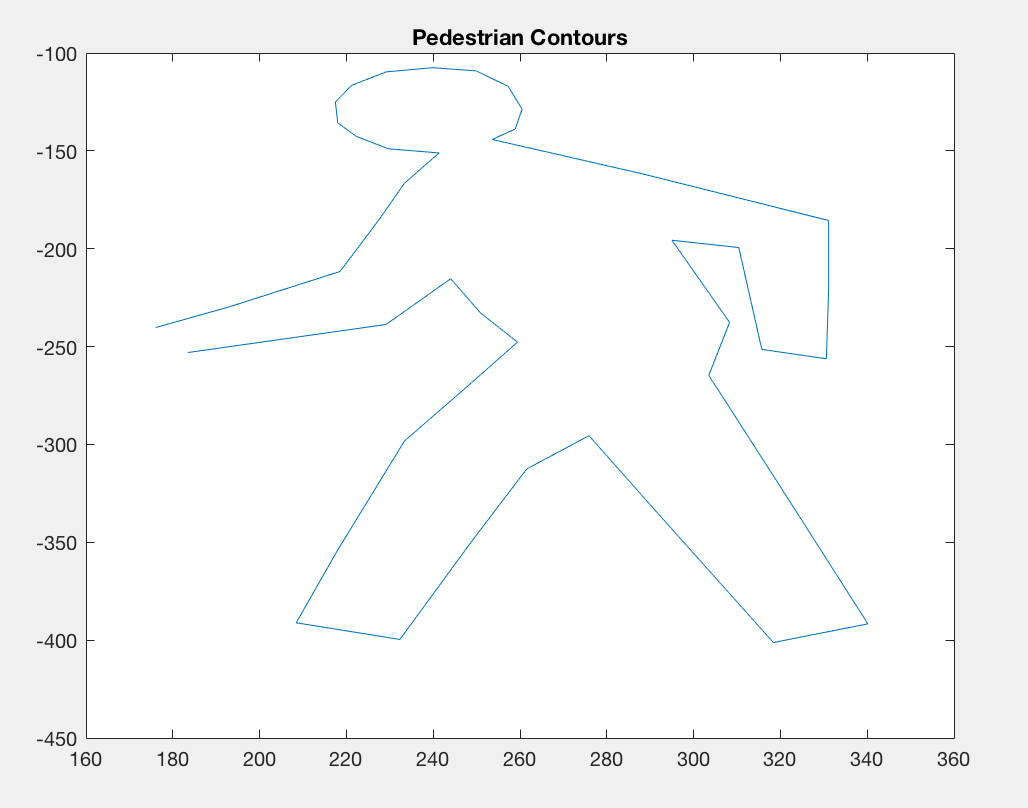
\includegraphics[height=5cm , width=8cm]{ped.jpg}

 \emph{Image showing contours of pedestrian image}
 \newline $b.$
\newline \emph{\textbf{Local Direction of Each Node Before Running Belief Propagation}}
\newline \begin{document}
\newline Flower Contours with Local evidence


 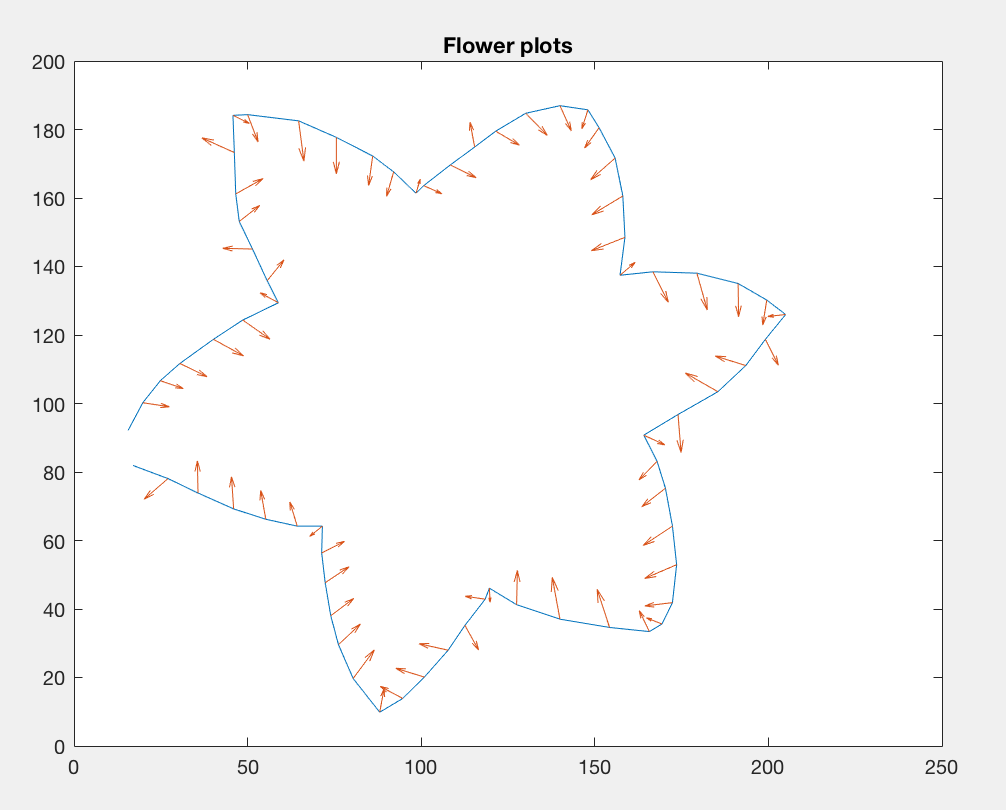
\includegraphics[height=5cm , width=8cm]{flower_cnt.png}
 
 
 \emph{Image showing flower contours with local evidence before belief propagation}
 \newline \begin{document}
\newline Hand Contours with Local Evidence

 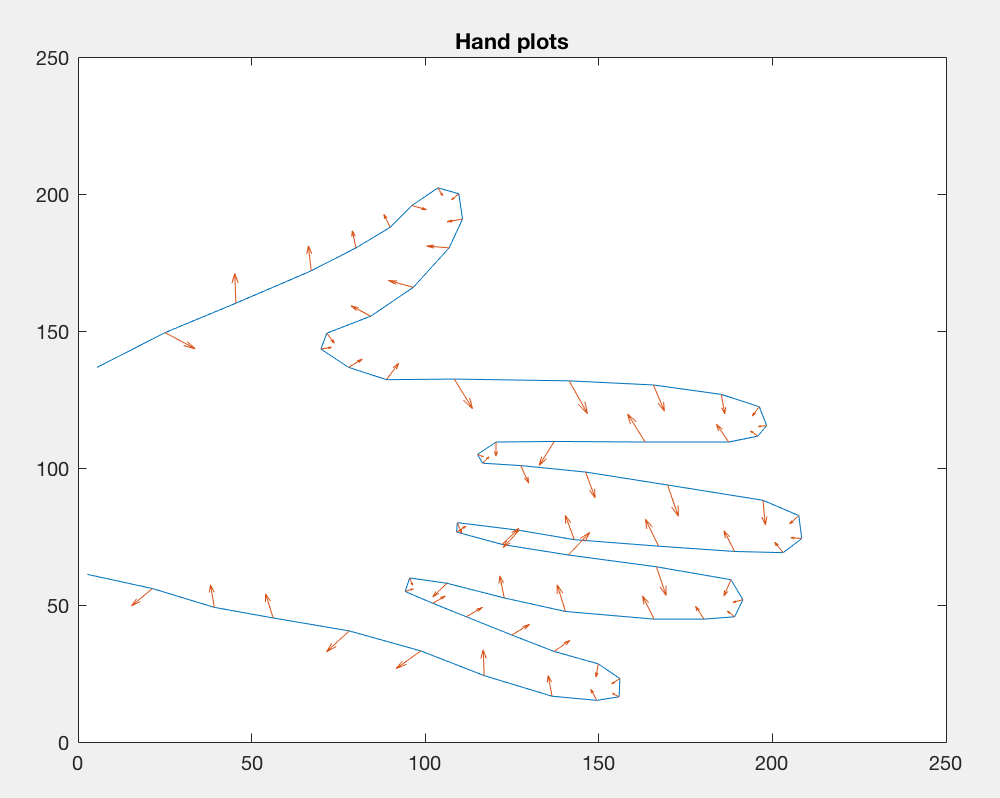
\includegraphics[height=5cm , width=8cm]{hand_cnt.png}

 \emph{Image showing hand contours with local evidence before belief propagation}
  \newline \begin{document}
\newline Pedestrian contours with Local Evidence

 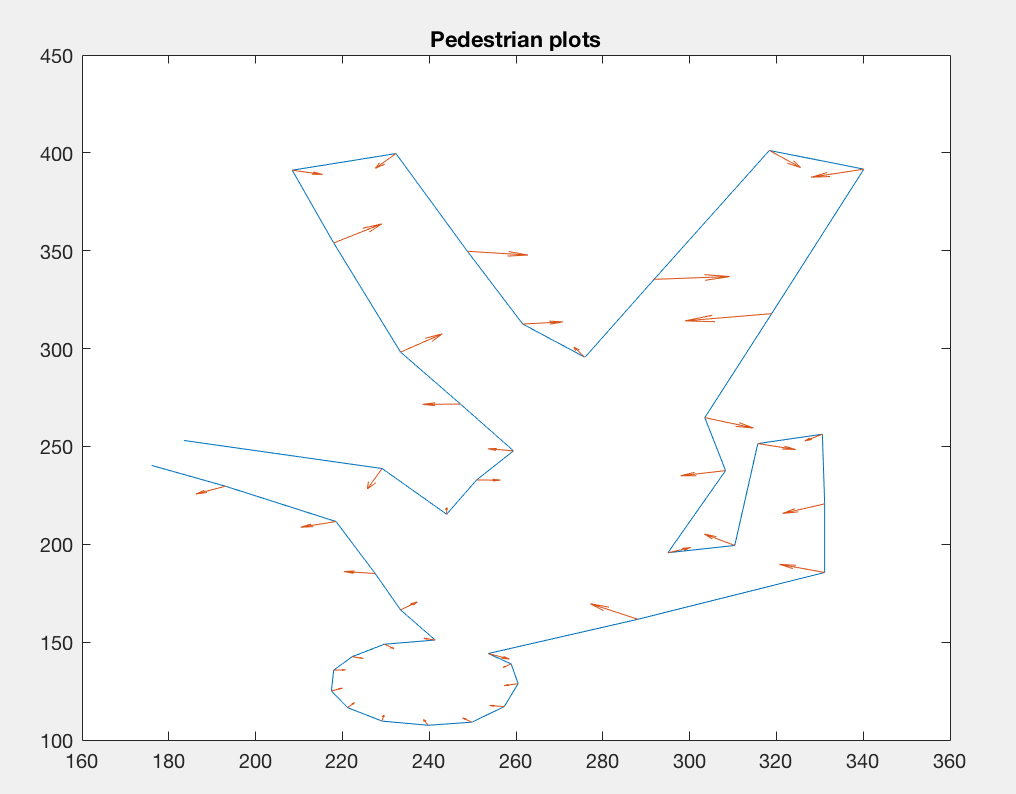
\includegraphics[height=5cm , width=8cm]{ped_cnt.png}

 \emph{Image showing pedestrian contours with local evidence before belief propagation}
\newline $c.$\emph{\textbf{Final Estimated Direction after Running Belief Propagation}}
\newline \emph{\textbf{Direction of Each Node After Belief Propagation}}
\newline \begin{document}
\newline Flower Contours with belief propagation


 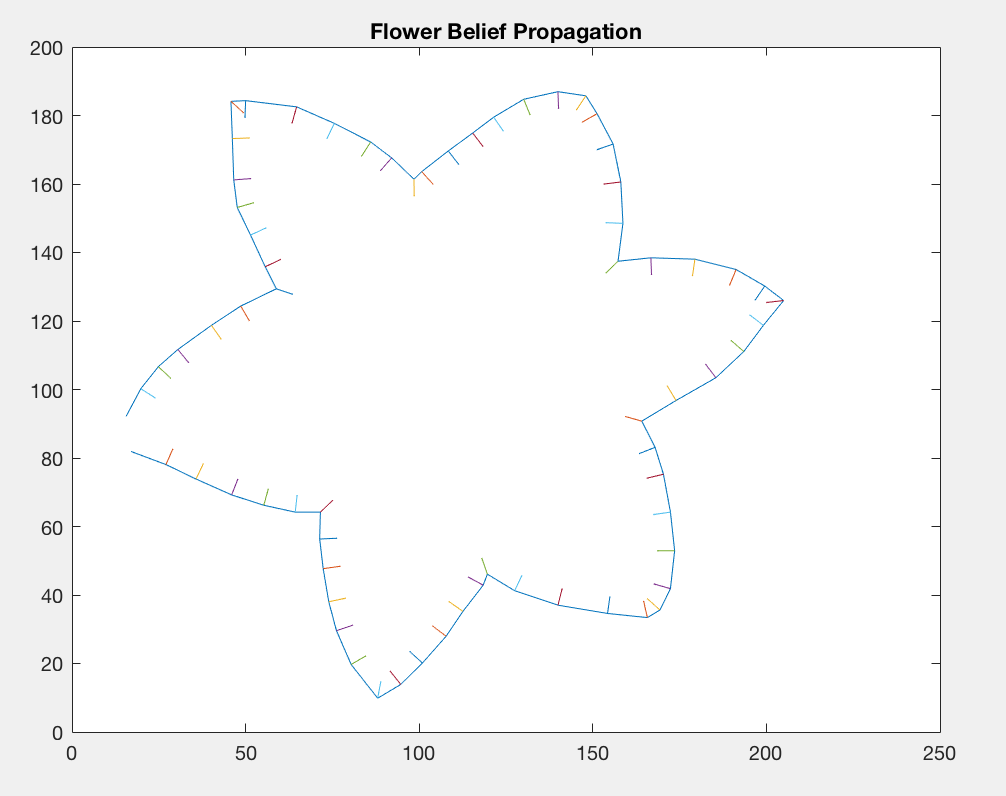
\includegraphics[height=5cm , width=8cm]{flower_blf.png}
 
 
 \emph{Image showing flower contours with belief propagation}
 \newline \begin{document}
\newline Hand Contours with belief propagation

 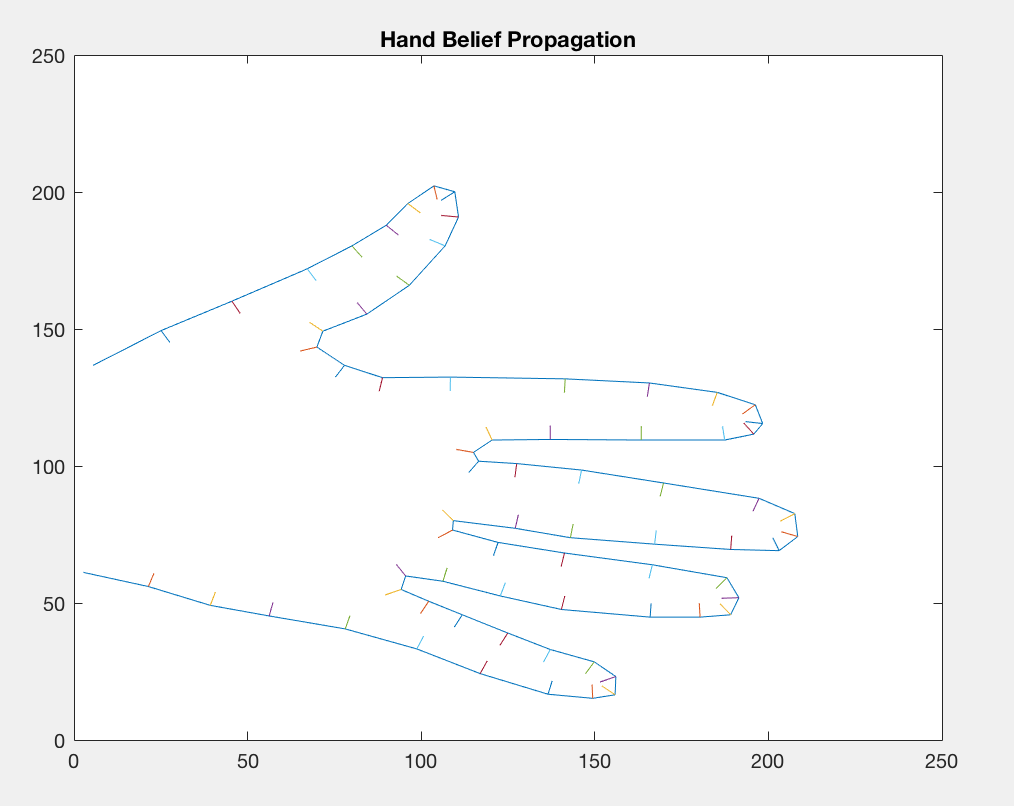
\includegraphics[height=5cm , width=8cm]{hand_blf.png}

 \emph{Image showing hand contours with belief propagation}
  \newline \begin{document}
\newline Pedestrian contours with Belief Propagation

 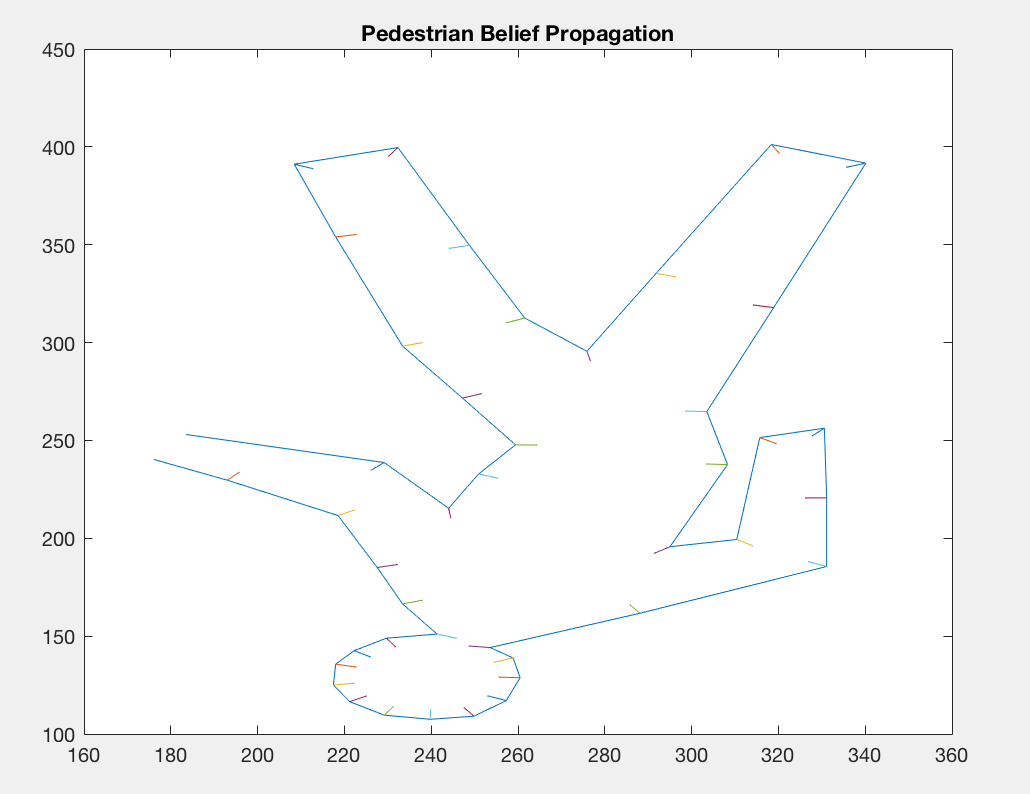
\includegraphics[height=5cm , width=8cm]{pedestrian_blf.png}

 \emph{Image showing pedestrian contours with belief propagation}
\end{document}